\section{Results}
\label{sec:Results}
%\subsection{Elastic Scattering}

A benchmark region of interest is defined between the upper and lower thresholds in cS1 for each channel. This region
is bounded in $y$-space from above by the $^{241}$AmBe NR mean line and below by the lower 3$\sigma$ quantile of the $^{241}$AmBe neutron calibration data. The expected background in the region is $3 \pm 0.5$ (low-energy) and $1.41 \pm 0.28$ (high-energy). The number of DM candidates in this benchmark region is 3 (low-energy), and 0 (high-energy). The data is compatible with the background-only hypothesis and no excess is found. 

For the elastic scattering case, a 90\%\,CL$_S$~\cite{cls} confidence level limit is set on the effective coupling constant, $c_i$,  for all operators and masses in the range of 10~GeV/$c^2$ to 1 TeV/$c^2$. The $c_i$ are dimensionful, with units of $[\mathrm{mass}]^{-2}$, so we first convert them to dimensionless quantities by multiplying them by $m_\mathrm{weak}^2=(246.2\text{ GeV})^2$, following the conventions of \cite{Anand:MathTools}. 
%\Xehund\ sets the strongest limits. % tomorrow another experiment will be better.
These limits are shown in Fig.~\ref{fig:elasticLimit} in black, along with limits from CDMS-II Si, CDMS-II Ge and SuperCDMS~\cite{CDMSEFT}.  

\begin{figure}
%\centerline{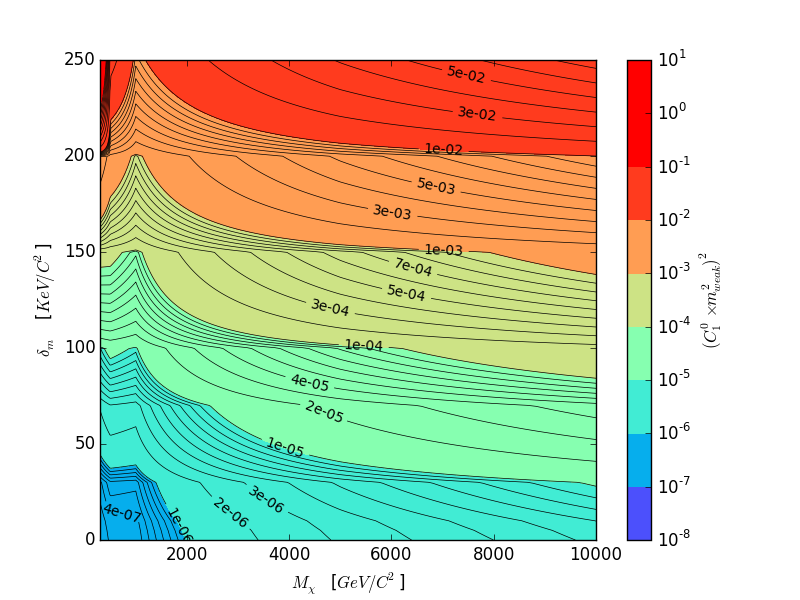
\includegraphics[width=1.\linewidth]{Figures/inelastic_delta_vs_m.png}}
\centerline{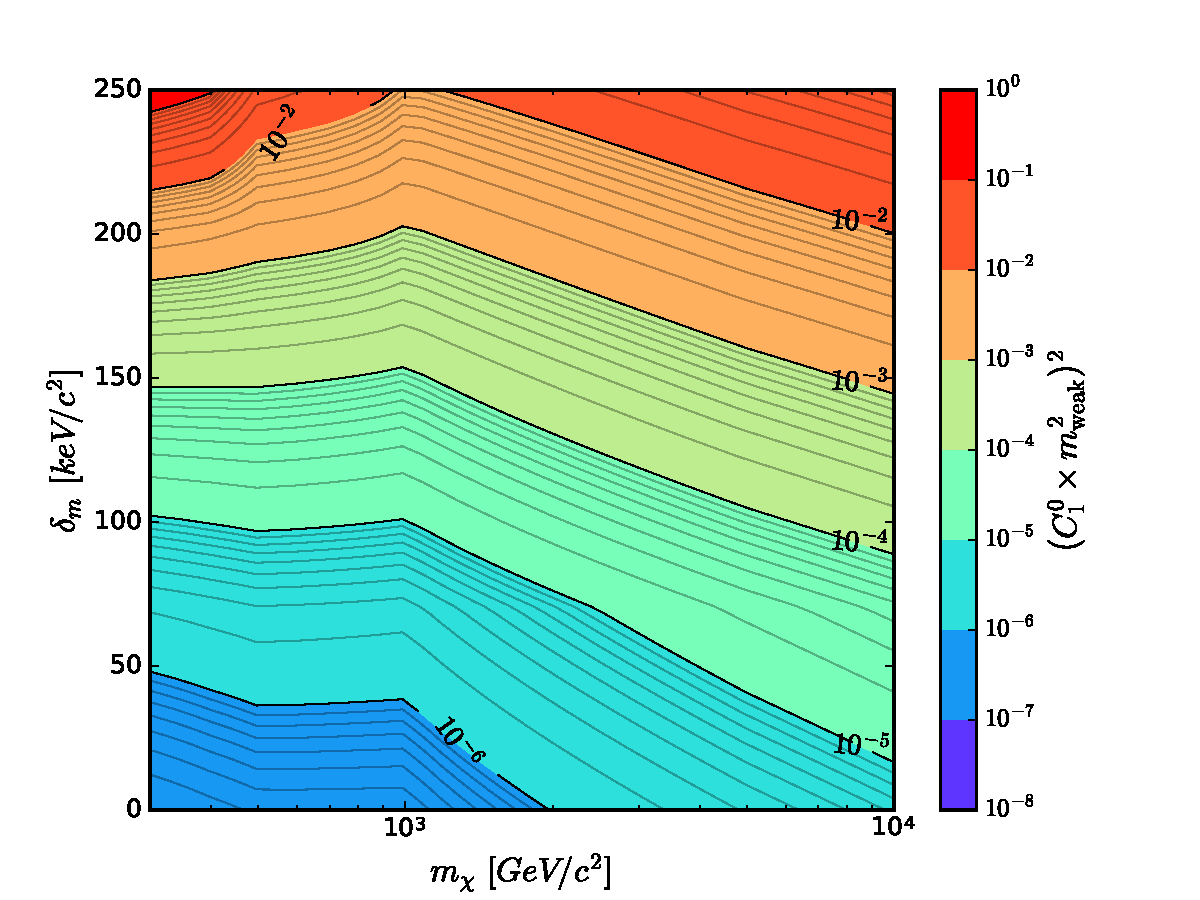
\includegraphics[width=1.\linewidth]{Figures/O1_inelastic_lim_2D}}
\caption{90\%\,CL$_S$ limits, for the inelastic model, on the magnitude of the coupling constant for $\mathcal{O}_1$, reported as a function of the WIMP mass and mass splitting $\delta$.}
\label{fig:O1Inel}
\end{figure}  

For the inelastic scattering case,  90\%\,CL$_S$ confidence level limits on the coupling constants 
(again scaled by $m_\mathrm{weak}^2$) are set. Fig.~\ref{fig:O1Inel} shows limits on the $\mathcal{O}_1$ (SI) coupling constant as a function of mass splitting and WIMP mass, Fig.~\ref{fig:InelasticLimit} shows limits for all other operators as a function of the mass splitting $\delta_m$ with a fixed WIMP mass of 1 TeV/$c^2$,  
projections of results from CDMS-II~\cite{CDMS_Inelastic}, Zepplin-III~\cite{Zepplin_Inel}, and Xenon100~\cite{XENON_Inelastic_WIMP} in the coupling constant and $\delta_m$ parameter space are also reported.
  

\begin{figure*}
\begin{minipage}{1.\linewidth}{}
\centerline{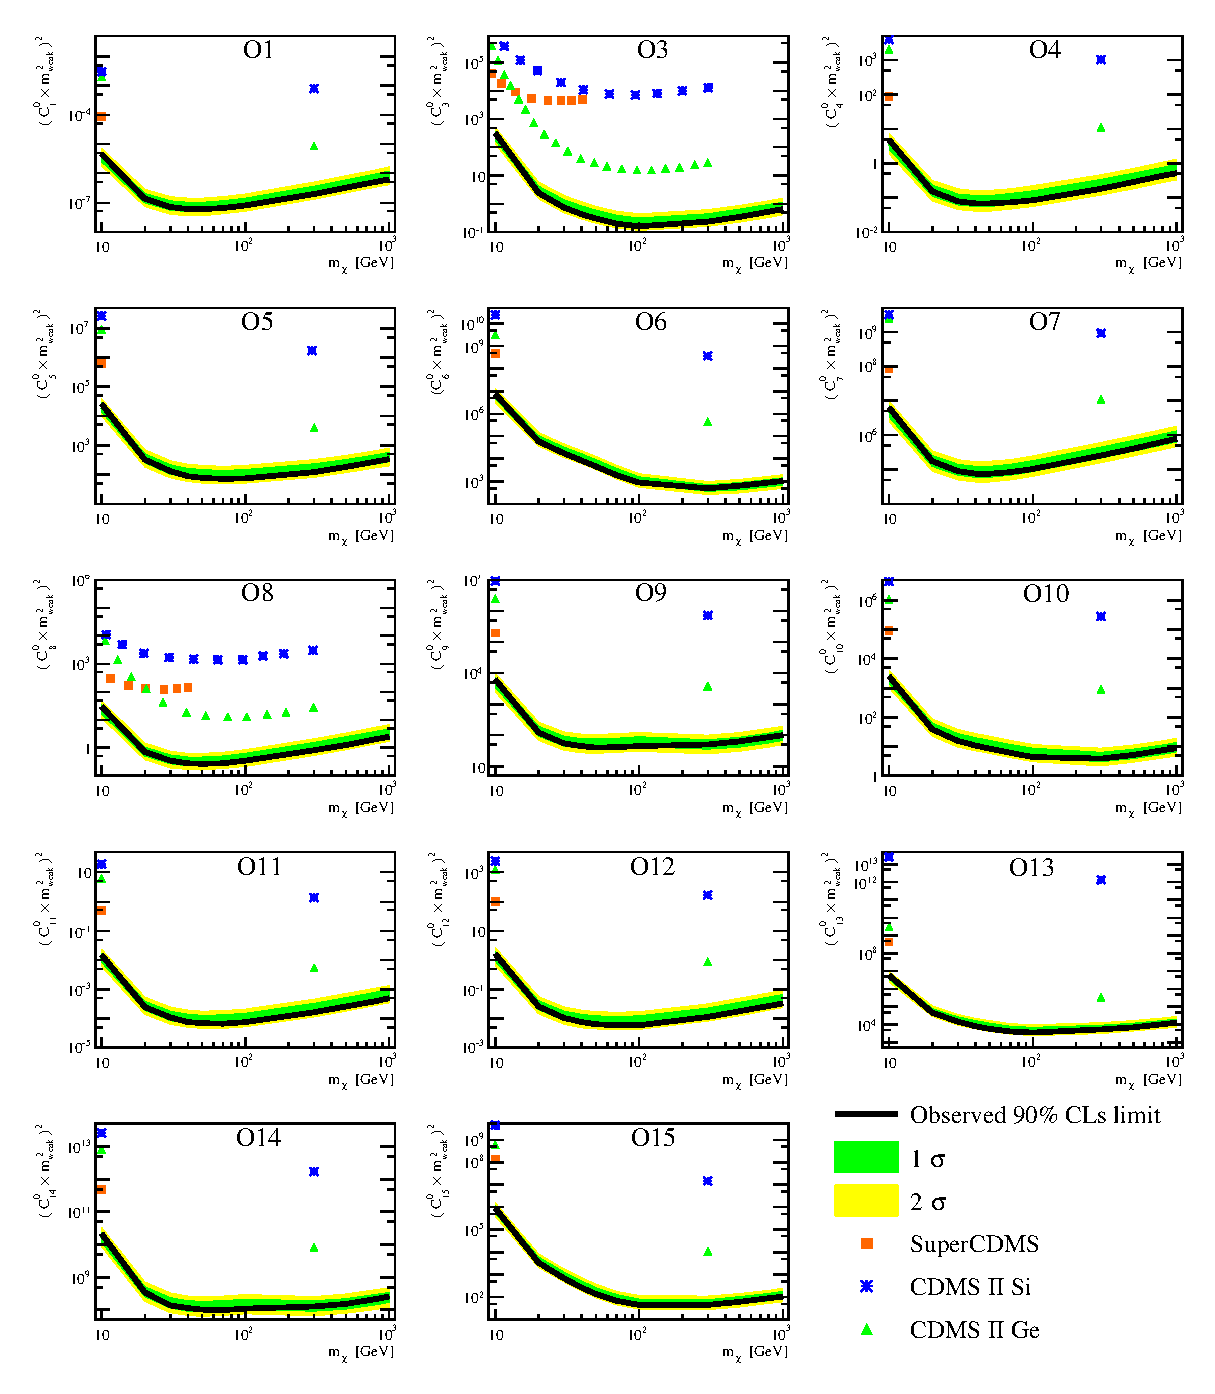
\includegraphics[width=\textwidth,height=0.99\textheight,keepaspectratio]{Figures/ElasticAllLimitCDMS.eps}}
\end{minipage}
\caption{The \Xehund\ limits (90\%\,CL$_S$) on isoscalar dimensionless coupling for all elastic scattering EFT operators. The limits are indicated in solid black. The expected sensitivity is shown in green and yellow(1$\sigma$ and 2$\sigma$ respectively). Limits from CDMS-II Si, CDMS-II Ge, and SuperCDMS \cite{CDMSEFT} are presented as blue asterisks, green triangles, and orange rectangles, respectively (color online). For operator 3 and 8 a full limit was published, for all other operators only $m_\chi = 10$ and $m_\chi =300$ are available.}
\label{fig:elasticLimit}
\end{figure*}

\begin{figure*}
\begin{minipage}{1.\linewidth}
\centerline{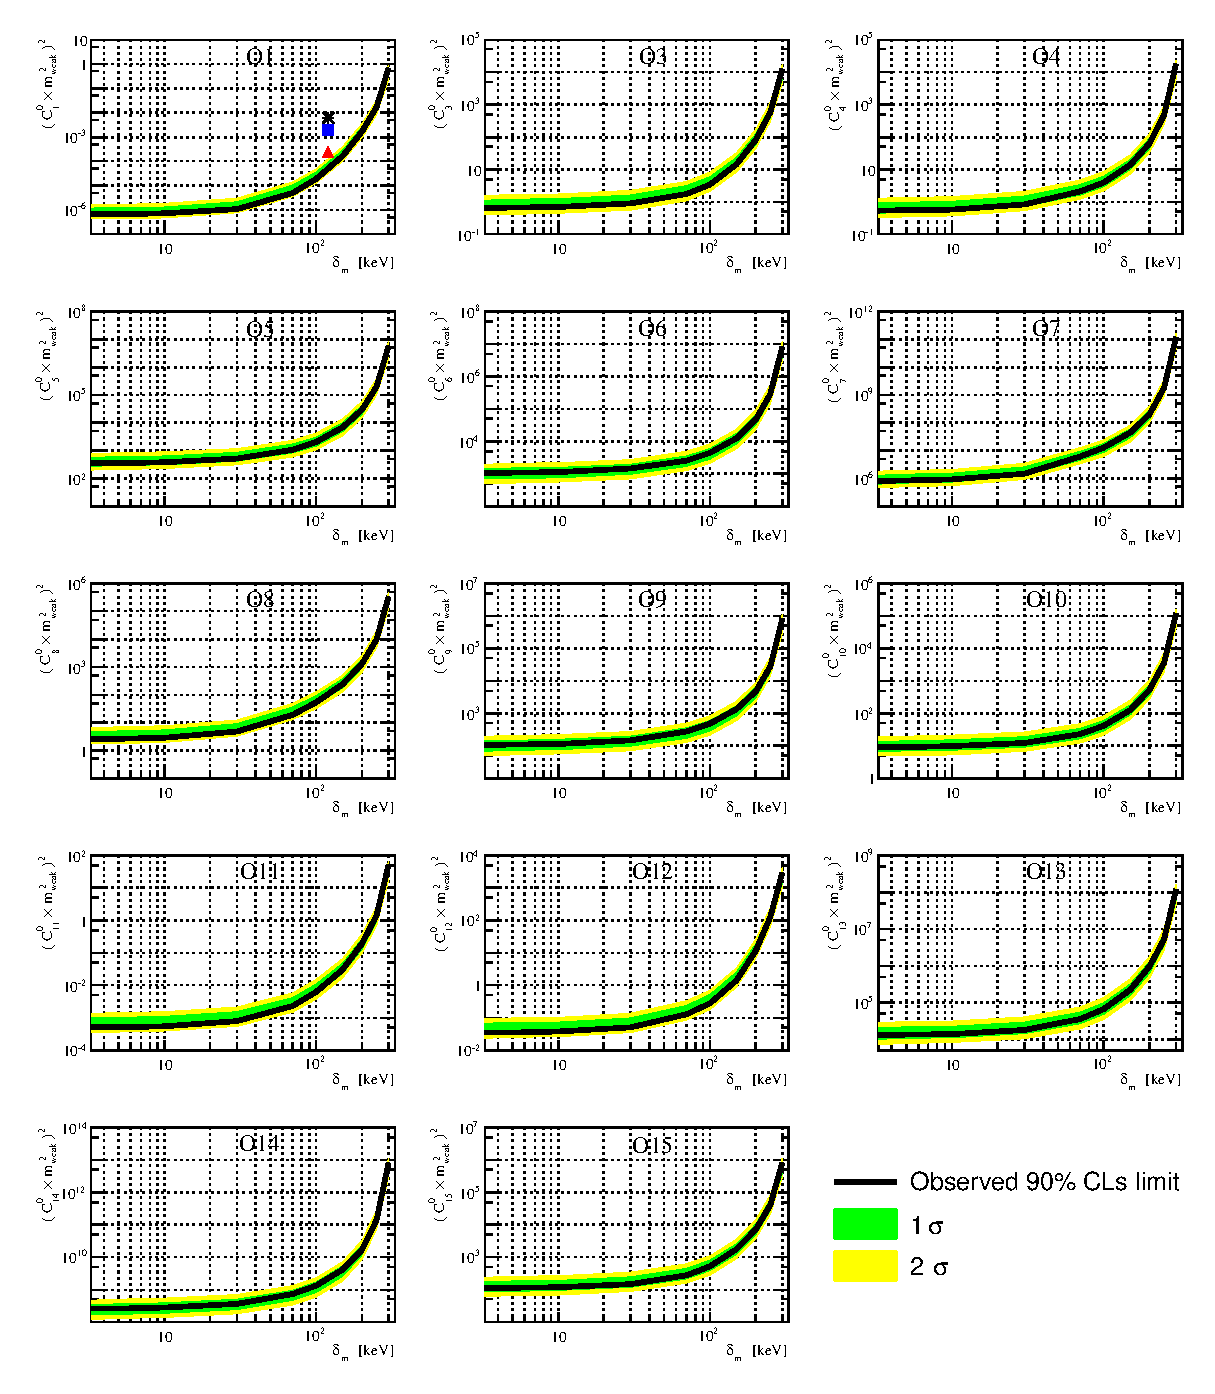
\includegraphics[width=\textwidth,height=0.99\textheight,keepaspectratio]{Figures/FinalInelastic.eps}}
\end{minipage}
\caption{The \Xehund\ 90\%\,CL$_S$ limits on a 1 TeV/$c^2$ WIMP isoscalar dimensionless coupling constant as function of the WIMP mass splitting $\delta_m$  for all inelastic scattering EFT operators. Limits are indicated in solid black. The expected sensitivity is shown in green and yellow (1$\sigma$ and 2$\sigma$ respectively). \RanComment{For $\mathcal{O}_1$ (SI) results from Xenon100(red triangle) CDMS-II(blue rectangle) and Zepplin-III)(black star) are overlaid (color online)}}
\label{fig:InelasticLimit}
\end{figure*}

Furthermore we examined the region in \cSi{} above 180\,PE and up to 1000\,PE. We used the same data selection criteria as those applied for the high-energy channel. 
In this energy regime, due to the lack of NR calibration data and of a rigorous background model, a quantitative and statistically solid inference on dark
matter hypoteses is impractical. Figure~\ref{fig:eft_1000}, shows the distribution of science data in this extended range togheter with NR and ER calibration data,
the two large populations (in black) at ~350\,PE and ~500\,PE are the 110\,keV and 197\,keV excitation lines of $^{19}$F coming from the PTFE walls of the TPC. 
There is no evidence for anomalies based on these data and the current knowledge.

\BenComment{For the elastic operator $O_1$ our results can be compared to those of standard SI analyses by computing the relevant zero-momentum WIMP-nucleon cross-sections. This is not simple to do rigorously because the treatment of nuclear structure used in our analysis is different than in standard analyses, however this difference is small for scattering via $O_1$. We can therefore quite safely use the `traditional' correspondence
%
\begin{equation}
\sigma_{N}^\mathrm{SI} = \left(C^N_1\right)^2 \frac{\mu_{\chi,N}^2}{\pi}
\end{equation}
%
where $\mu_{\chi,N}$ is the WIMP-nucleon reduced mass. Standard SI analyses assume isospin-conserving interactions, as we do in this analysis, so we can simply set $C^N_1 = C^0_1$, such that $\sigma_{p}^\mathrm{SI}=\sigma_{n}^\mathrm{SI}$. 
}

\BenComment{In principle a similar comparison can be done between our limit on the $O_4$ coupling and standard SD analysis limits, however this time the standard analyses do {\em not} assume isospin-conserving interactions. Instead they typically assume maximal isospin violation, that is, assuming that WIMPs couple only to either protons or neutrons. Limits are then derived independently on $\sigma_{p}^\mathrm{SD}$ and $\sigma_{n}^\mathrm{SD}$. Because of this difference in assumptions, our limits on SD couplings are not directly comparable to usual analyses, though they can be recast under the appropriate alternate model assumptions using the detector response tables we provide in Appendix~\ref{app:response_table}.
}

\begin{figure}
\centerline{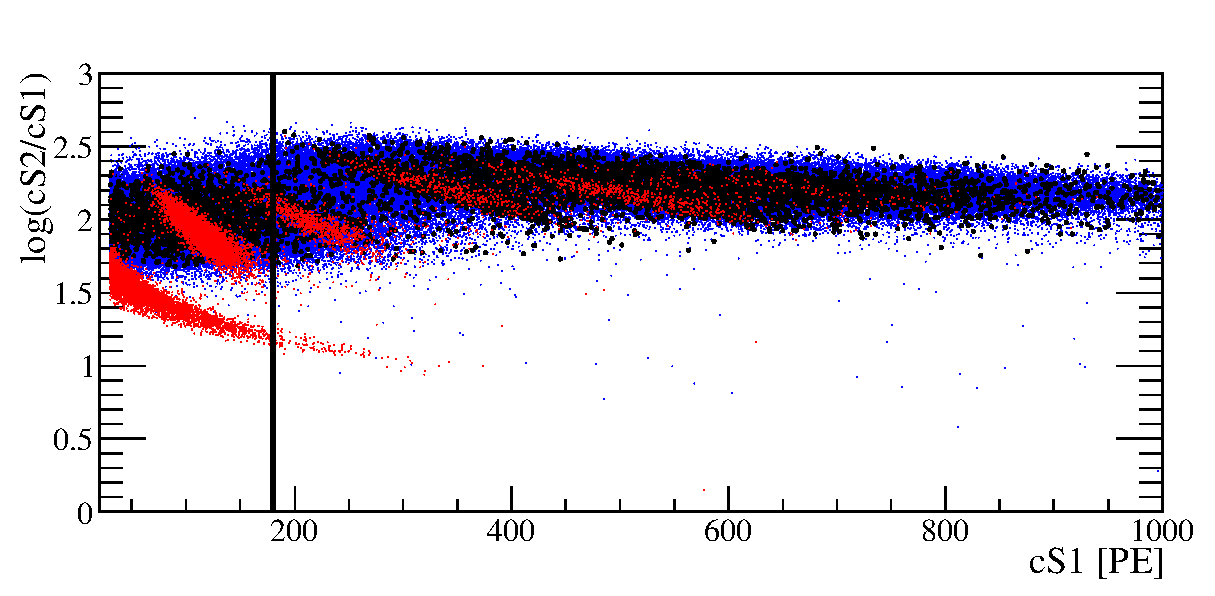
\includegraphics[width=1.\linewidth]
{Figures/allDataFullScale.eps}}
\caption{The full \Xehund{} dark matter science run data up to 1000~PE in \cSi{} (shown in black). In blue we show data from ER calibration ($^{60}$Co and $^{232}$Th). In red we show data from NR calibration ($^{241}$AmBe). The two large populations (in black) at ~350\,PE and ~500\,PE are the 110\,keV and 197\,keV excitation lines of $^{19}$F coming from the PTFE walls of the TPC. \RanComment{The black vertical line represents the highest energy considered for this analysis.} 
%No statistical analysis is possible for the data above about 180~PE in \cSi{}, due to insufficient NR calibration sample statistics. However, from the trend of the calibration data and the lack of candidate events outside the ER band, we can heuristically claim to see zero candidate nuclear recoil events in the energy regime beyond our analysis.
}
\label{fig:eft_1000}
\end{figure}  




% \begin{figure*}
% \begin{minipage}{1.\linewidth}
% \centerline{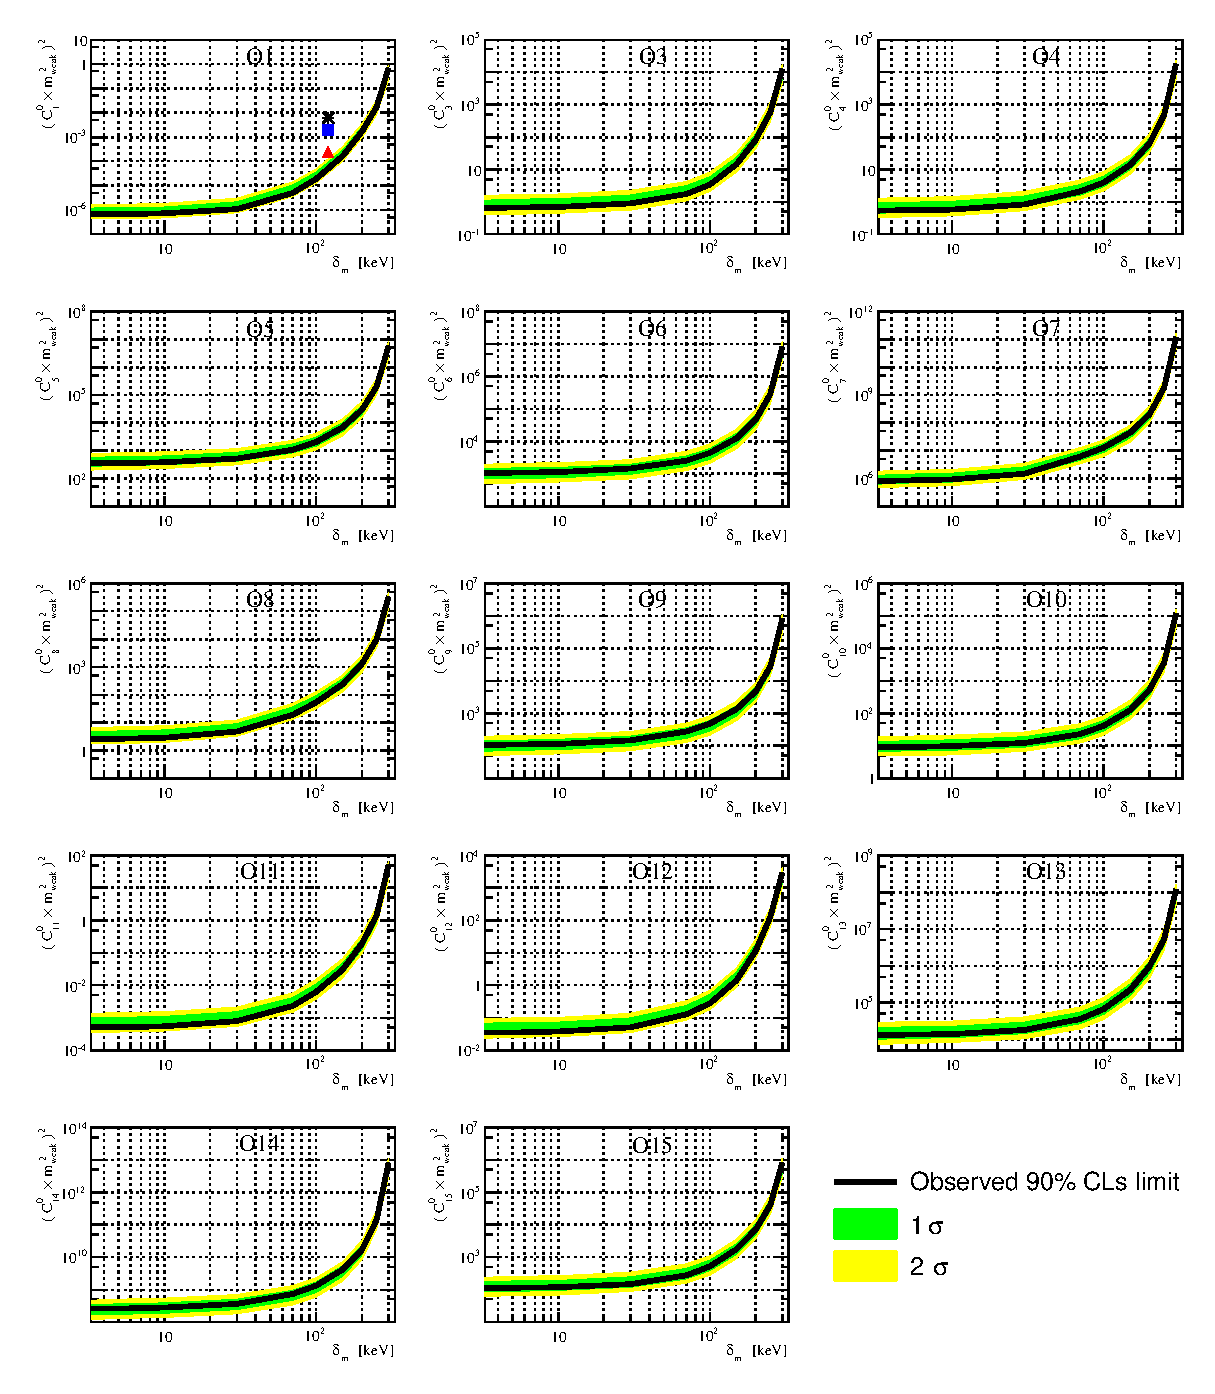
\includegraphics[width=\textwidth,height=0.95\textheight,keepaspectratio]{Figures/FinalInelastic.eps}}
% \end{minipage}
% \caption{The \Xehund\ 90\%\,CL$_S$ limits on a 1 TeV/$c^2$ WIMP isoscalar dimensionless coupling for all inelastic scattering EFT operators. Limits are indicated in solid black. The expected sensitivity is shown in green and yellow (1$\sigma$ and 2$\sigma$ respectively).}
% \label{fig:InelasticLimit}
% \end{figure*}

%\FloatBarrier

